%%%%%%%%%%%%%%%%%%%%%%%%%%%%%%%%%%%%%%%%%
% Beamer Presentation
% LaTeX Template
% Version 1.0 (10/11/12)
%
% This template has been downloaded from:
% http://www.LaTeXTemplates.com
%
% License:
% CC BY-NC-SA 3.0 (http://creativecommons.org/licenses/by-nc-sa/3.0/)
%
%%%%%%%%%%%%%%%%%%%%%%%%%%%%%%%%%%%%%%%%%

%----------------------------------------------------------------------------------------
%	PACKAGES AND THEMES
%----------------------------------------------------------------------------------------

\documentclass[UTF8,aspectratio=169,14pt]{ctexbeamer}

\usepackage{hyperref}
\hypersetup{
	colorlinks=true,
	linkcolor=red,
	anchorcolor=blue,
	citecolor=green
}

\mode<presentation> {
	
	% The Beamer class comes with a number of default slide themes
	% which change the colors and layouts of slides. Below this is a list
	% of all the themes, uncomment each in turn to see what they look like.
	
	%\usetheme{default}
	%\usetheme{AnnArbor}
	%\usetheme{Antibes}
	%\usetheme{Bergen}
	%\usetheme{Berkeley}
	%\usetheme{Berlin}
	%\usetheme{Boadilla}
	%\usetheme{CambridgeUS}
	%\usetheme{Copenhagen}
	%\usetheme{Darmstadt}
	%\usetheme{Dresden}
	%\usetheme{Frankfurt}
	%\usetheme{Goettingen}
	%\usetheme{Hannover}
	%\usetheme{Ilmenau}
	%\usetheme{JuanLesPins}
	%\usetheme{Luebeck}
	\usetheme{Madrid}
	%\usetheme{Malmoe}
	%\usetheme{Marburg}
	%\usetheme{Montpellier}
	%\usetheme{PaloAlto}
	%\usetheme{Pittsburgh}
	%\usetheme{Rochester}
	%\usetheme{Singapore}
	%\usetheme{Szeged}
	%\usetheme{Warsaw}
	
	% As well as themes, the Beamer class has a number of color themes
	% for any slide theme. Uncomment each of these in turn to see how it
	% changes the colors of your current slide theme.
	
	%\usecolortheme{albatross}
	%\usecolortheme{beaver}
	%\usecolortheme{beetle}
	%\usecolortheme{crane}
	%\usecolortheme{dolphin}
	%\usecolortheme{dove}
	%\usecolortheme{fly}
	%\usecolortheme{lily}
	%\usecolortheme{orchid}
	%\usecolortheme{rose}
	%\usecolortheme{seagull}
	%\usecolortheme{seahorse}
	%\usecolortheme{whale}
	%\usecolortheme{wolverine}
	
	%\setbeamertemplate{footline} % To remove the footer line in all slides uncomment this line
	%\setbeamertemplate{footline}[page number] % To replace the footer line in all slides with a simple slide count uncomment this line
	
	%\setbeamertemplate{navigation symbols}{} % To remove the navigation symbols from the bottom of all slides uncomment this line
}

\usepackage{graphicx} % Allows including images
\graphicspath{{./figs/}}
\usepackage{booktabs} % Allows the use of \toprule, \midrule and \bottomrule in tables
\usepackage{longtable}
\usepackage{listings}
\usepackage{xcolor}
\lstset{numbers=left, %设置行号位置
	numberstyle=\tiny, %设置行号大小
	keywordstyle=\color{blue}, %设置关键字颜色
	commentstyle=\color[cmyk]{1,0,1,0}, %设置注释颜色
	frame=single, %设置边框格式
	escapeinside=``, %逃逸字符(1左面的键),用于显示中文
	%breaklines, %自动折行
	extendedchars=false, %解决代码跨页时,章节标题,页眉等汉字不显示的问题
	xleftmargin=2em,xrightmargin=2em, aboveskip=1em, %设置边距
	tabsize=4, %设置tab空格数
	showspaces=false %不显示空格
}
% Fonts
% \usepackage{libertine}
% \setmonofont{Courier}
\setCJKsansfont[ItalicFont=Noto Serif CJK SC Black, BoldFont=Noto Sans CJK SC Black]{Noto Sans CJK SC}


%----------------------------------------------------------------------------------------
%   TITLE PAGE
%----------------------------------------------------------------------------------------

\title[第6讲]{第六讲 虚拟存储概念} % The short title appears at the bottom of every slide, the full title is only on the title page
\subtitle{第4节 RISC-V缺页异常}
\author{向勇、陈渝、李国良} % Your name
\institute[清华大学] % Your institution as it will appear on the bottom of every slide, may be shorthand to save space
{
清华大学计算机系 \\ % Your institution for the title page
\medskip
\textit{xyong,yuchen,liguoliang@tsinghua.edu.cn} % Your email address
}
\date{\today} % Date, can be changed to a custom date

\begin{document}

\begin{frame}
\titlepage % Print the title page as the first slide
\end{frame}

%----------------------------------------------------------------------------------------
\begin{frame}
\frametitle{提纲} % Table of contents slide, comment this block out to remove it
\tableofcontents % Throughout your presentation, if you choose to use \section{} and \subsection{} commands, these will automatically be printed on this slide as an overview of your presentation
\end{frame}
%----------------------------------------------------------------------------------------
%   PRESENTATION SLIDES
%----------------------------------------------------------------------------------------
%------------------------------------------------
\section{第4节 RISC-V缺页异常}% Sections can be created in order to organize your presentation into discrete blocks, all sections and subsections are automatically printed in the table of contents as an overview of the talk
%------------------------------------------------
\subsection{内核态的中断处理机制回顾} % A subsection can be created just before a set of slides with a common theme to further break down your presentation into chunks


%------------------------------------------------
\begin{frame}[fragile,plain]
	\frametitle{内核态的中断处理机制回顾}
	\begin{figure}
	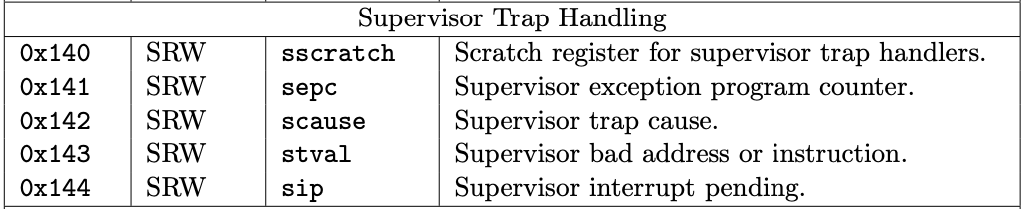
\includegraphics[width=1.0\linewidth]{SupervisorTrapHandling}
	\end{figure}
\end{frame}
%riscv-privileged-v1.10.pdf
%page 20
%
%Supervisor Trap Handling
%与中断相关的寄存器
%
%![SupervisorTrapHandling](/Users/xyong/Desktop/figs/SupervisorTrapHandling.png)
%
%
%
%At the beginning of a trap handler, sscratch is swapped with a user register to provide an initial working register.
%
%When a trap is taken into S-mode, sepc is written with the virtual address of the instruction that encountered the exception.
%
%The Interrupt bit in the scause register is set if the contains a code identifying the last exception.
%
%When a hardware breakpoint is triggered, or an instruction-fetch, load, or store access or page-fault exception occurs, or an instruction-fetch or AMO address-misaligned exception occurs, stval is written with the faulting address.
%
%The sip register is an XLEN-bit read/write register containing information on pending interrupts, while sie is the corresponding XLEN-bit read/write register containing interrupt enable bits.
%------------------------------------------------
\begin{frame}[fragile,plain]   
	\frametitle{中断原因寄存器(scause)}
	\begin{figure}
	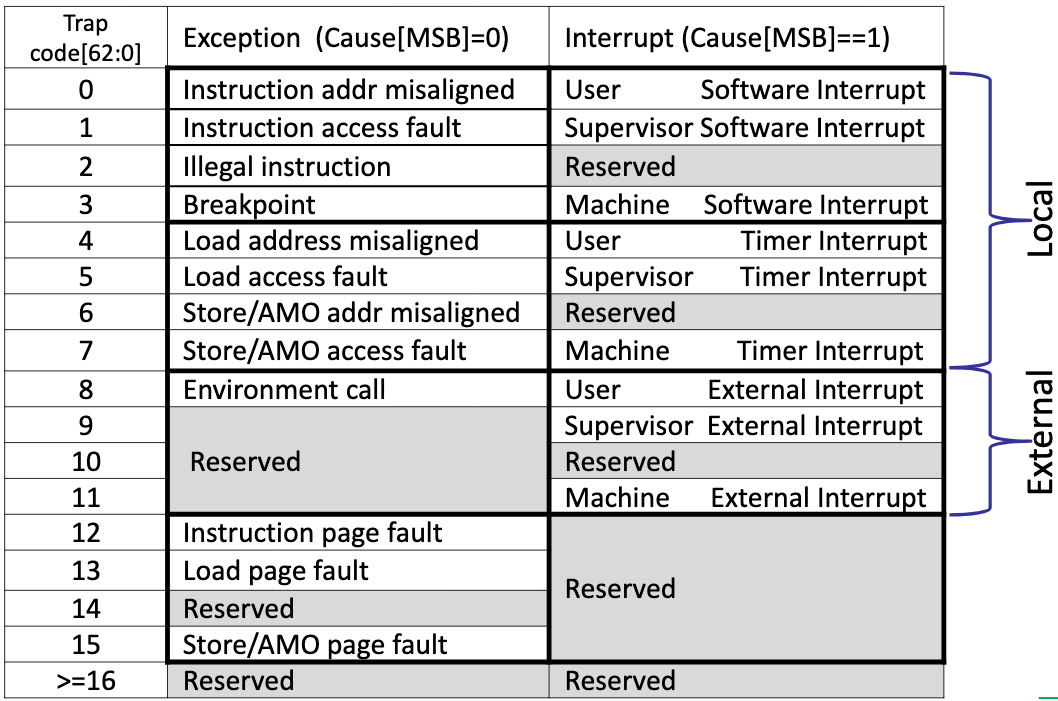
\includegraphics[width=0.75\linewidth]{scause-CSR}
	\end{figure}
\end{frame}
%https://content.riscv.org/wp-content/uploads/2018/05/riscv-privileged-BCN.v7-2.pdf
%Page 25
%
%![scause-CSR](/Users/xyong/Desktop/figs/scause-CSR.png)
%------------------------------------------------
\subsection{RISC-V缺页异常}
%------------------------------------------------
\begin{frame}[fragile,plain]   
	\frametitle{\href{https://content.riscv.org/wp-content/uploads/2017/05/riscv-privileged-v1.10.pdf}{Volume II: RISC-V Privileged Architectures V1.10}}
	\begin{figure}
	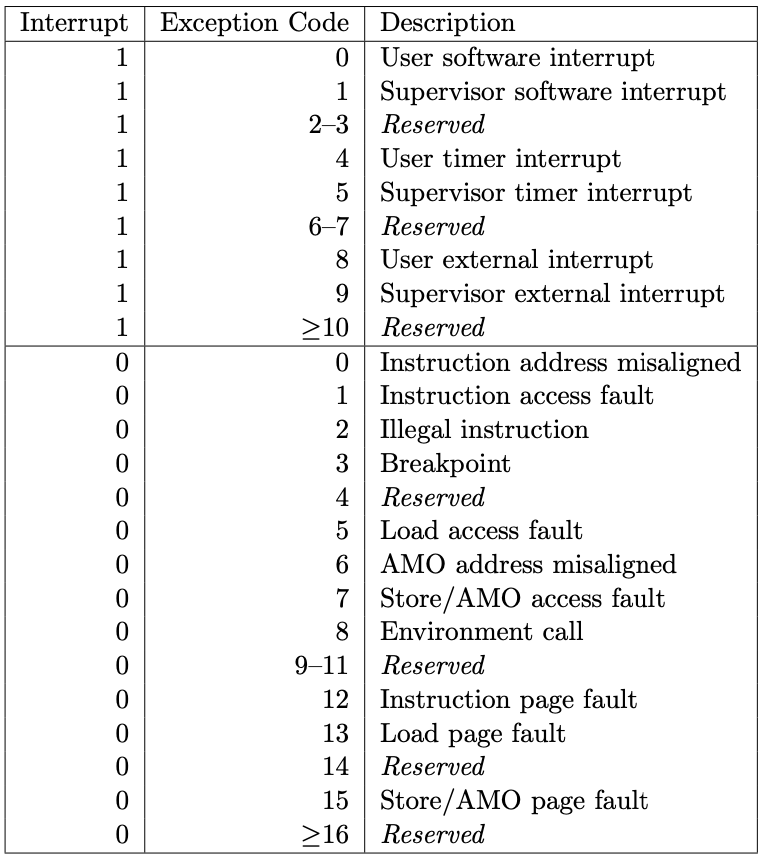
\includegraphics[width=0.4\linewidth]{scause-trap.png}
	\caption{Supervisor cause register (scause) values after trap}
	\end{figure}
\end{frame}
% ### Supervisor cause register (scause) values after trap
% 
% riscv-privileged-v1.10.pdf
% page 65
% Table 4.2: Supervisor cause register (scause) values after trap.
% 
% Instruction access
% Load access fault
% 
% ![scause-trap](/Users/xyong/Desktop/figs/scause-trap.png)
%------------------------------------------------
\begin{frame}[fragile,plain]   
	\frametitle{rCore的缺页异常处理}
    \begin{itemize}
        \item 缺页异常只会在 MMU 启用后,虚拟地址翻译失败时产生,这时候根据是取指还是访存,分别触发 不同的缺页异常。 \pause
        \item 当状态码是 Instruction page fault、Load page fault、Store page fault 时,将被判断为是缺页异常,并调用 `handle\_page\_fault()` 处理缺页异常。 \pause
        \item 发生缺页异常时,虚拟地址将会被保存到stval寄存器中;再调用 `crate::memory::page\_fault\_handler(addr)` 来做具体的缺页处理。\pause
        \item 出处:rCore (Commit ID \href{https://github.com/rcore-os/rCore/tree/cd81f4cc73ea3302ed0356398525b0b56c4fca92}{cd81f4c})
    \end{itemize}
\end{frame}
% ### rCore的缺页异常处理
% 
% Ref: rCore-2_OSLab-g2-interrupt.md-缺页异常
% 
% 缺页异常只会在 MMU 启用后,虚拟地址翻译失败时产生,这时候根据是取指还是访存,分别触发 Instruction Abort 与 Data Abort。
% 
% 当状态码是 translation fault、access flag fault、permission fault 时,将被判断为是缺页异常,并调用 `handle_page_fault()` 处理缺页异常。
% 
% 发生 Instruction page fault 和 Load/Store page access时,虚拟地址将会被保存到stval寄存器中;再调用 `crate::memory::page_fault_handler(addr)` 来做具体的缺页处理。
%------------------------------------------------
\subsection{rCore中的RISC-V缺页异常处理函数}
%------------------------------------------------
\begin{frame}[fragile,plain]   
	\frametitle{rCore中RISC-V的缺页处理函数handle\_page\_fault}
    \begin{itemize}
        \item \href{https://github.com/rcore-os/rCore/blob/cd81f4cc73ea3302ed0356398525b0b56c4fca92/kernel/src/arch/riscv/interrupt.rs#L56}{kernel/src/arch/riscv/interrupt.rs}
\begin{verbatim}
fn rust_trap(tf: &mut TrapFrame)
\end{verbatim} \pause
        \item \href{https://github.com/rcore-os/rCore/blob/cd81f4cc73ea3302ed0356398525b0b56c4fca92/kernel/src/arch/riscv/interrupt.rs#L125}{kernel/src/arch/riscv/interrupt.rs}
\begin{verbatim}
fn page_fault(tf: &mut TrapFrame)
\end{verbatim} \pause
        \item \href{https://github.com/rcore-os/rCore/blob/cd81f4cc73ea3302ed0356398525b0b56c4fca92/kernel/src/memory.rs\#L132}{kernel/src/memory.rs}
\begin{verbatim}
pub fn handle_page_fault(addr: usize) -> bool
\end{verbatim} \pause
        \item \href{https://github.com/rcore-os/rCore/blob/master/crate/memory/src/memory_set/mod.rs#L379}{crate/memory/src/memory\_set/mod.rs}
\begin{verbatim}
pub fn handle_page_fault(&mut self, addr: VirtAddr) -> bool
\end{verbatim}
\pause
        \item \href{https://github.com/rcore-os/rCore/blob/master/crate/memory/src/memory_set/handler/delay.rs#L52}{crate/memory/src/memory\_set/handler/delay.rs}
\begin{verbatim}
fn handle_page_fault(&self, pt: &mut dyn PageTable, addr: VirtAddr) -> bool
\end{verbatim}
    \end{itemize}
\end{frame}
% ### handle_page_fault
% 
% fn rust_trap(tf: &mut TrapFrame)
% 
% fn page_fault(tf: &mut TrapFrame)
% 
% pub fn handle_page_fault(addr: usize) -> bool
% 
% pub fn handle_page_fault(&mut self, addr: VirtAddr) -> bool
% 
% fn handle_page_fault(&self, pt: &mut dyn PageTable, addr: VirtAddr) -> bool
% 
% let frame = self.allocator.alloc().expect("failed to alloc frame");
% entry.set_target(frame);
% entry.set_present(true);
% entry.update();
%------------------------------------------------
\begin{frame}[fragile,plain]   
	\frametitle{crate/memory/src/memory\_set/handler/delay.rs}
\begin{verbatim}
fn handle_page_fault(&self, pt: &mut dyn PageTable, addr: VirtAddr) -> bool
\end{verbatim}
\begin{block}{}
\begin{verbatim}
......
let frame = self.allocator.alloc().expect("failed to alloc frame");
                          ///分配物理页面
entry.set_target(frame);  ///设置物理页号
entry.set_present(true);  ///设置页表项标志位
entry.update();           ///TLB刷新
......
\end{verbatim}
\end{block}
\end{frame}
%------------------------------------------------
\end{document}
